\documentclass[twoside]{book}

% Packages required by doxygen
\usepackage{fixltx2e}
\usepackage{calc}
\usepackage{doxygen}
\usepackage[export]{adjustbox} % also loads graphicx
\usepackage{graphicx}
\usepackage[utf8]{inputenc}
\usepackage{makeidx}
\usepackage{multicol}
\usepackage{multirow}
\PassOptionsToPackage{warn}{textcomp}
\usepackage{textcomp}
\usepackage[nointegrals]{wasysym}
\usepackage[table]{xcolor}

% NLS support packages
\usepackage[T2A]{fontenc}
\usepackage[russian]{babel}

% Font selection
\usepackage[T1]{fontenc}
\usepackage[scaled=.90]{helvet}
\usepackage{courier}
\usepackage{amssymb}
\usepackage{sectsty}
\renewcommand{\familydefault}{\sfdefault}
\allsectionsfont{%
  \fontseries{bc}\selectfont%
  \color{darkgray}%
}
\renewcommand{\DoxyLabelFont}{%
  \fontseries{bc}\selectfont%
  \color{darkgray}%
}
\newcommand{\+}{\discretionary{\mbox{\scriptsize$\hookleftarrow$}}{}{}}

% Page & text layout
\usepackage{geometry}
\geometry{%
  a4paper,%
  top=2.5cm,%
  bottom=2.5cm,%
  left=2.5cm,%
  right=2.5cm%
}
\tolerance=750
\hfuzz=15pt
\hbadness=750
\setlength{\emergencystretch}{15pt}
\setlength{\parindent}{0cm}
\setlength{\parskip}{3ex plus 2ex minus 2ex}
\makeatletter
\renewcommand{\paragraph}{%
  \@startsection{paragraph}{4}{0ex}{-1.0ex}{1.0ex}{%
    \normalfont\normalsize\bfseries\SS@parafont%
  }%
}
\renewcommand{\subparagraph}{%
  \@startsection{subparagraph}{5}{0ex}{-1.0ex}{1.0ex}{%
    \normalfont\normalsize\bfseries\SS@subparafont%
  }%
}
\makeatother

% Headers & footers
\usepackage{fancyhdr}
\pagestyle{fancyplain}
\fancyhead[LE]{\fancyplain{}{\bfseries\thepage}}
\fancyhead[CE]{\fancyplain{}{}}
\fancyhead[RE]{\fancyplain{}{\bfseries\leftmark}}
\fancyhead[LO]{\fancyplain{}{\bfseries\rightmark}}
\fancyhead[CO]{\fancyplain{}{}}
\fancyhead[RO]{\fancyplain{}{\bfseries\thepage}}
\fancyfoot[LE]{\fancyplain{}{}}
\fancyfoot[CE]{\fancyplain{}{}}
\fancyfoot[RE]{\fancyplain{}{\bfseries\scriptsize Создано системой Doxygen }}
\fancyfoot[LO]{\fancyplain{}{\bfseries\scriptsize Создано системой Doxygen }}
\fancyfoot[CO]{\fancyplain{}{}}
\fancyfoot[RO]{\fancyplain{}{}}
\renewcommand{\footrulewidth}{0.4pt}
\renewcommand{\chaptermark}[1]{%
  \markboth{#1}{}%
}
\renewcommand{\sectionmark}[1]{%
  \markright{\thesection\ #1}%
}

% Indices & bibliography
\usepackage{natbib}
\usepackage[titles]{tocloft}
\setcounter{tocdepth}{3}
\setcounter{secnumdepth}{5}
\makeindex

% Hyperlinks (required, but should be loaded last)
\usepackage{ifpdf}
\ifpdf
  \usepackage[pdftex,pagebackref=true]{hyperref}
\else
  \usepackage[ps2pdf,pagebackref=true]{hyperref}
\fi
\hypersetup{%
  colorlinks=true,%
  linkcolor=blue,%
  citecolor=blue,%
  unicode%
}

% Custom commands
\newcommand{\clearemptydoublepage}{%
  \newpage{\pagestyle{empty}\cleardoublepage}%
}

\usepackage{caption}
\captionsetup{labelsep=space,justification=centering,font={bf},singlelinecheck=off,skip=4pt,position=top}

%===== C O N T E N T S =====

\begin{document}

% Titlepage & ToC
\hypersetup{pageanchor=false,
             bookmarksnumbered=true,
             pdfencoding=unicode
            }
\pagenumbering{alph}
\begin{titlepage}
\vspace*{7cm}
\begin{center}%
{\Large Toxic-\/\+Comment-\/\+Classification }\\
\vspace*{1cm}
{\large Создано системой Doxygen 1.8.14}\\
\end{center}
\end{titlepage}
\clearemptydoublepage
\pagenumbering{roman}
\tableofcontents
\clearemptydoublepage
\pagenumbering{arabic}
\hypersetup{pageanchor=true}

%--- Begin generated contents ---
\chapter{Иерархический список классов}
\section{Иерархия классов}
Иерархия классов.\begin{DoxyCompactList}
\item \contentsline{section}{Controller}{\pageref{class_controller}}{}
\begin{DoxyCompactList}
\item \contentsline{section}{Main\+Controller}{\pageref{class_main_controller}}{}
\end{DoxyCompactList}
\item \contentsline{section}{Core}{\pageref{class_core}}{}
\item \contentsline{section}{Data\+Processing}{\pageref{class_data_processing}}{}
\item \contentsline{section}{Data\+Provider}{\pageref{class_data_provider}}{}
\begin{DoxyCompactList}
\item \contentsline{section}{File\+Data\+Provider}{\pageref{class_file_data_provider}}{}
\end{DoxyCompactList}
\item \contentsline{section}{Message}{\pageref{class_message}}{}
\end{DoxyCompactList}

\chapter{Алфавитный указатель классов}
\section{Классы}
Классы с их кратким описанием.\begin{DoxyCompactList}
\item\contentsline{section}{\mbox{\hyperlink{class_controller}{Controller}} \\*Интерфейс для классов контроллеров управляющими ходом программы }{\pageref{class_controller}}{}
\item\contentsline{section}{\mbox{\hyperlink{class_core}{Core}} \\*Интерфейс классов ядра для определения \char`\"{}недоброжелательности\char`\"{} текста }{\pageref{class_core}}{}
\item\contentsline{section}{\mbox{\hyperlink{class_data_processing}{Data\+Processing}} \\*Интерфейс для классов предобработки текста }{\pageref{class_data_processing}}{}
\item\contentsline{section}{\mbox{\hyperlink{class_data_provider}{Data\+Provider}} \\*Интерфейс для классов считывания/записи данных }{\pageref{class_data_provider}}{}
\item\contentsline{section}{\mbox{\hyperlink{class_file_data_provider}{File\+Data\+Provider}} \\*Класс для считывания/записи данных из/в файл(а) }{\pageref{class_file_data_provider}}{}
\item\contentsline{section}{\mbox{\hyperlink{class_main_controller}{Main\+Controller}} \\*Основной класс контроллер управляющий ходом программы }{\pageref{class_main_controller}}{}
\item\contentsline{section}{\mbox{\hyperlink{class_message}{Message}} }{\pageref{class_message}}{}
\end{DoxyCompactList}

\chapter{Классы}
\hypertarget{class_controller}{}\section{Класс Controller}
\label{class_controller}\index{Controller@{Controller}}


Интерфейс для классов контроллеров управляющими ходом программы  




{\ttfamily \#include $<$Controller.\+h$>$}

Граф наследования\+:Controller\+:\begin{figure}[H]
\begin{center}
\leavevmode
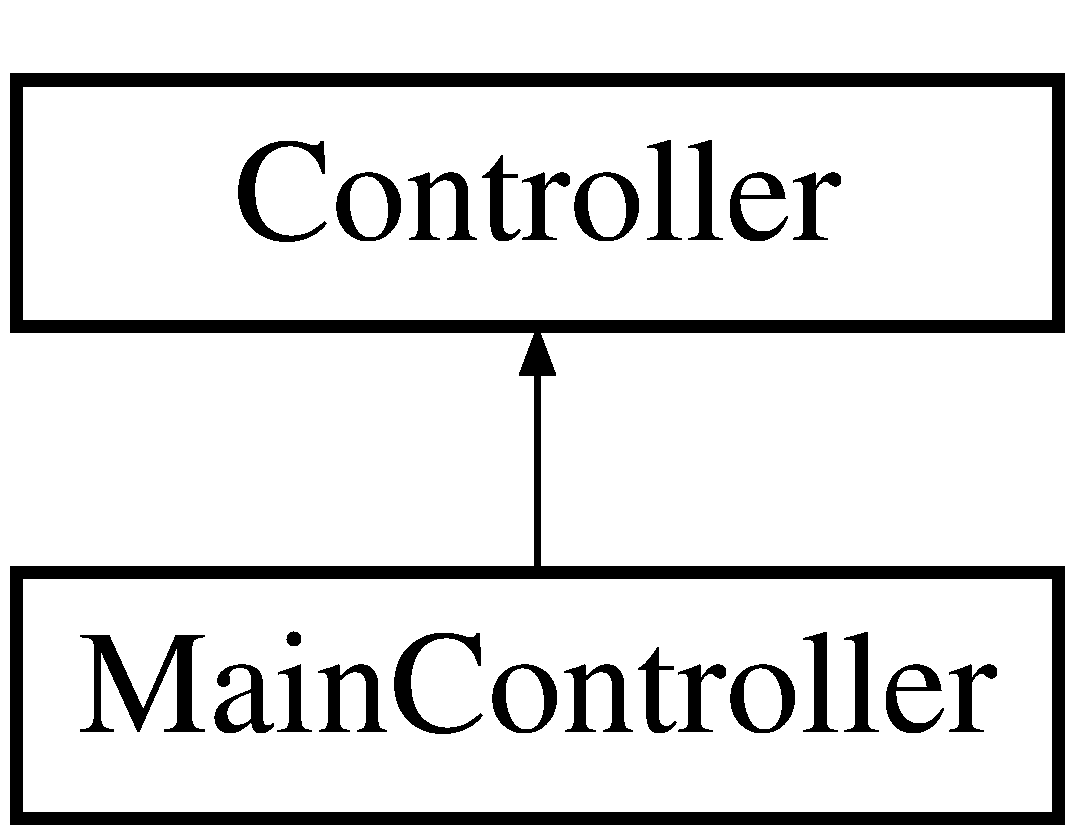
\includegraphics[height=2.000000cm]{class_controller}
\end{center}
\end{figure}


\subsection{Подробное описание}
Интерфейс для классов контроллеров управляющими ходом программы 

См. определение в файле Controller.\+h строка 10



Объявления и описания членов класса находятся в файле\+:\begin{DoxyCompactItemize}
\item 
Controllers/Controller.\+h\end{DoxyCompactItemize}

\hypertarget{class_core}{}\section{Класс Core}
\label{class_core}\index{Core@{Core}}


Интерфейс классов ядра для определения \char`\"{}недоброжелательности\char`\"{} текста  




{\ttfamily \#include $<$Core.\+h$>$}



\subsection{Подробное описание}
Интерфейс классов ядра для определения \char`\"{}недоброжелательности\char`\"{} текста 

См. определение в файле Core.\+h строка 8



Объявления и описания членов класса находятся в файле\+:\begin{DoxyCompactItemize}
\item 
Cores/Core.\+h\end{DoxyCompactItemize}

\hypertarget{class_data_processing}{}\section{Класс Data\+Processing}
\label{class_data_processing}\index{Data\+Processing@{Data\+Processing}}


Интерфейс для классов предобработки текста  




{\ttfamily \#include $<$Data\+Handler.\+h$>$}



\subsection{Подробное описание}
Интерфейс для классов предобработки текста 

См. определение в файле Data\+Handler.\+h строка 8



Объявления и описания членов класса находятся в файле\+:\begin{DoxyCompactItemize}
\item 
Data\+Handlers/Data\+Handler.\+h\end{DoxyCompactItemize}

\hypertarget{class_data_provider}{}\section{Класс Data\+Provider}
\label{class_data_provider}\index{Data\+Provider@{Data\+Provider}}


Интерфейс для классов считывания/записи данных  




{\ttfamily \#include $<$Data\+Provider.\+h$>$}

Граф наследования\+:Data\+Provider\+:\begin{figure}[H]
\begin{center}
\leavevmode
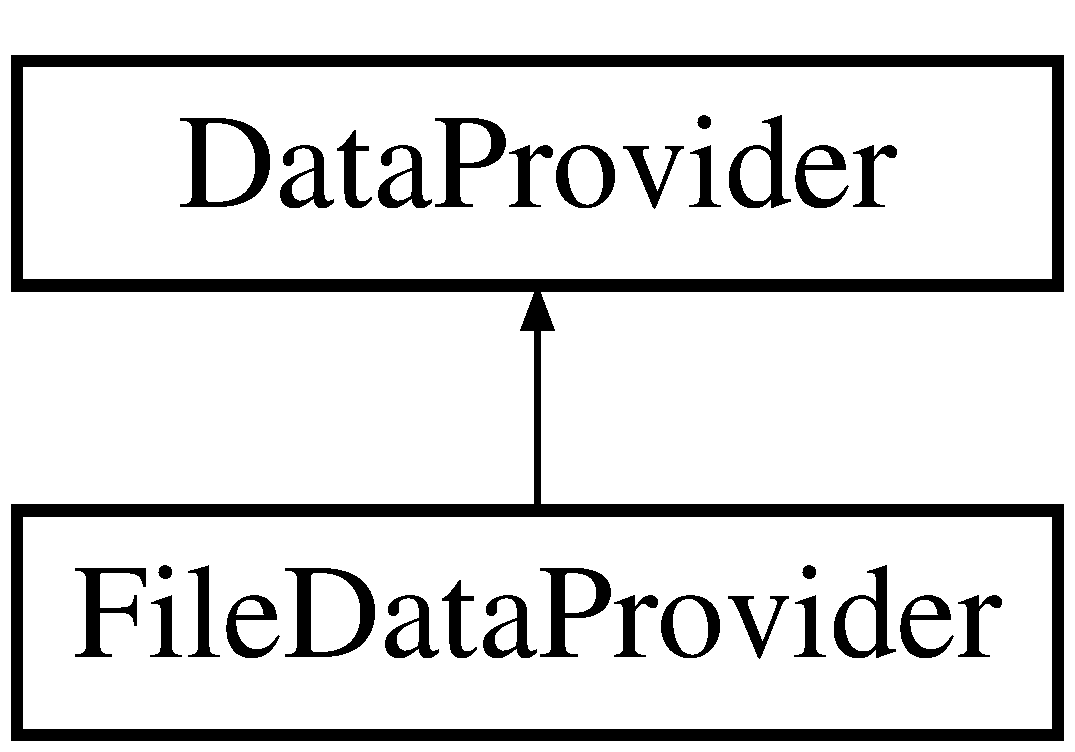
\includegraphics[height=2.000000cm]{class_data_provider}
\end{center}
\end{figure}


\subsection{Подробное описание}
Интерфейс для классов считывания/записи данных 

См. определение в файле Data\+Provider.\+h строка 10



Объявления и описания членов класса находятся в файле\+:\begin{DoxyCompactItemize}
\item 
Data\+Providers/Data\+Provider.\+h\end{DoxyCompactItemize}

\hypertarget{class_file_data_provider}{}\section{Класс File\+Data\+Provider}
\label{class_file_data_provider}\index{File\+Data\+Provider@{File\+Data\+Provider}}


Класс для считывания/записи данных из/в файл(а)  




{\ttfamily \#include $<$Data\+Provider.\+h$>$}

Граф наследования\+:File\+Data\+Provider\+:\begin{figure}[H]
\begin{center}
\leavevmode
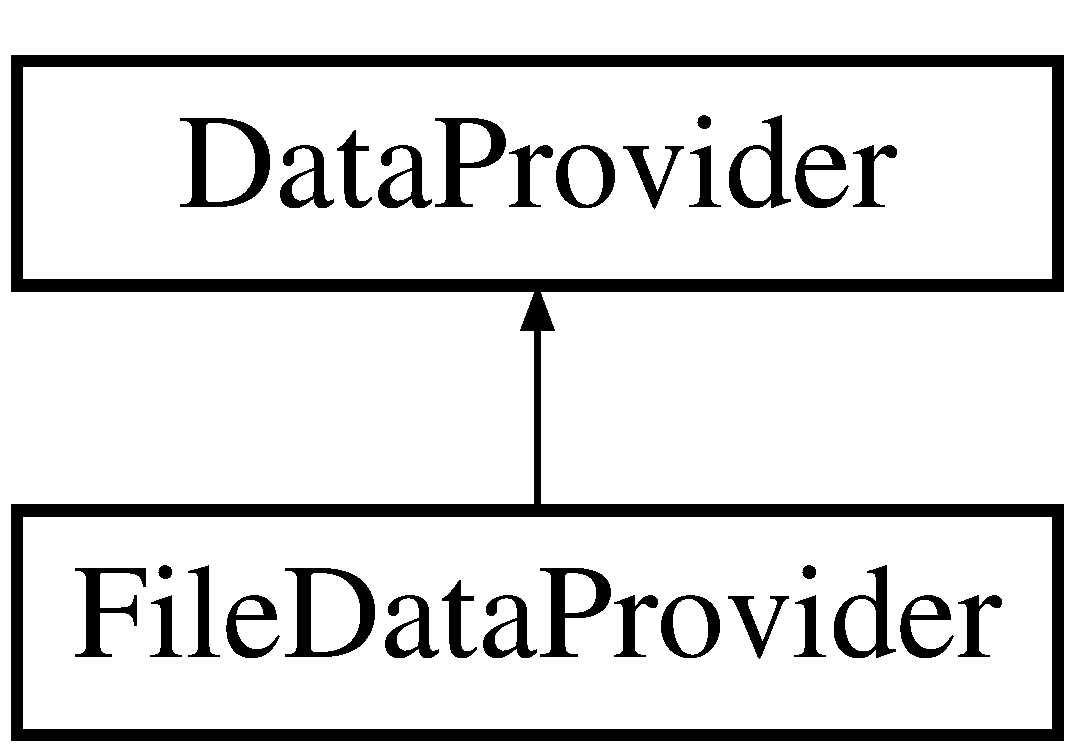
\includegraphics[height=2.000000cm]{class_file_data_provider}
\end{center}
\end{figure}
\subsection*{Открытые члены}
\begin{DoxyCompactItemize}
\item 
\mbox{\hyperlink{class_file_data_provider_a993b0c05a33d57eeb96c9269fc4479a5}{File\+Data\+Provider}} (std\+::vector$<$ char $>$ input\+\_\+file, std\+::vector$<$ char $>$ output\+\_\+file)
\begin{DoxyCompactList}\small\item\em Конструктор класса \end{DoxyCompactList}\item 
std\+::vector$<$ \mbox{\hyperlink{class_message}{Message}} $>$ \mbox{\hyperlink{class_file_data_provider_a3804f90fbca39fb9d9fa62389152a1a5}{get\+\_\+data}} () const override
\begin{DoxyCompactList}\small\item\em Функция для считывания данных из файла \end{DoxyCompactList}\item 
bool \mbox{\hyperlink{class_file_data_provider_aff73a92f2e079094d7b0b0c9829b1ead}{save\+\_\+data}} (const \mbox{\hyperlink{class_message}{Message}} \&msg) const override
\begin{DoxyCompactList}\small\item\em Функция для записи данных в файл \end{DoxyCompactList}\end{DoxyCompactItemize}


\subsection{Подробное описание}
Класс для считывания/записи данных из/в файл(а) 

См. определение в файле Data\+Provider.\+h строка 30



\subsection{Конструктор(ы)}
\mbox{\Hypertarget{class_file_data_provider_a993b0c05a33d57eeb96c9269fc4479a5}\label{class_file_data_provider_a993b0c05a33d57eeb96c9269fc4479a5}} 
\index{File\+Data\+Provider@{File\+Data\+Provider}!File\+Data\+Provider@{File\+Data\+Provider}}
\index{File\+Data\+Provider@{File\+Data\+Provider}!File\+Data\+Provider@{File\+Data\+Provider}}
\subsubsection{\texorpdfstring{File\+Data\+Provider()}{FileDataProvider()}}
{\footnotesize\ttfamily File\+Data\+Provider\+::\+File\+Data\+Provider (\begin{DoxyParamCaption}\item[{std\+::vector$<$ char $>$}]{input\+\_\+file,  }\item[{std\+::vector$<$ char $>$}]{output\+\_\+file }\end{DoxyParamCaption})\hspace{0.3cm}{\ttfamily [inline]}}



Конструктор класса 


\begin{DoxyParams}{Аргументы}
{\em input\+\_\+file} & Имя файла для чтения \\
\hline
{\em output\+\_\+file} & Имя файла для записи \\
\hline
\end{DoxyParams}


См. определение в файле Data\+Provider.\+h строка 41



\subsection{Методы}
\mbox{\Hypertarget{class_file_data_provider_a3804f90fbca39fb9d9fa62389152a1a5}\label{class_file_data_provider_a3804f90fbca39fb9d9fa62389152a1a5}} 
\index{File\+Data\+Provider@{File\+Data\+Provider}!get\+\_\+data@{get\+\_\+data}}
\index{get\+\_\+data@{get\+\_\+data}!File\+Data\+Provider@{File\+Data\+Provider}}
\subsubsection{\texorpdfstring{get\+\_\+data()}{get\_data()}}
{\footnotesize\ttfamily std\+::vector$<$\mbox{\hyperlink{class_message}{Message}}$>$ File\+Data\+Provider\+::get\+\_\+data (\begin{DoxyParamCaption}{ }\end{DoxyParamCaption}) const\hspace{0.3cm}{\ttfamily [override]}, {\ttfamily [virtual]}}



Функция для считывания данных из файла 

\begin{DoxyReturn}{Возвращает}
Вектор структур данных, содержащих в себе считанные данные 
\end{DoxyReturn}

\begin{DoxyExceptions}{Исключения}
{\em I\+O\+Exception} & Исключение возникающее при проблемах с чтением файла \\
\hline
\end{DoxyExceptions}


Замещает \mbox{\hyperlink{class_data_provider}{Data\+Provider}}.

\mbox{\Hypertarget{class_file_data_provider_aff73a92f2e079094d7b0b0c9829b1ead}\label{class_file_data_provider_aff73a92f2e079094d7b0b0c9829b1ead}} 
\index{File\+Data\+Provider@{File\+Data\+Provider}!save\+\_\+data@{save\+\_\+data}}
\index{save\+\_\+data@{save\+\_\+data}!File\+Data\+Provider@{File\+Data\+Provider}}
\subsubsection{\texorpdfstring{save\+\_\+data()}{save\_data()}}
{\footnotesize\ttfamily bool File\+Data\+Provider\+::save\+\_\+data (\begin{DoxyParamCaption}\item[{const \mbox{\hyperlink{class_message}{Message}} \&}]{msg }\end{DoxyParamCaption}) const\hspace{0.3cm}{\ttfamily [override]}, {\ttfamily [virtual]}}



Функция для записи данных в файл 


\begin{DoxyParams}{Аргументы}
{\em msg} & Структура данных, содержащая в себе данные подлежащие записи \\
\hline
\end{DoxyParams}
\begin{DoxyReturn}{Возвращает}
Булевое значение\+:
\begin{DoxyItemize}
\item 0 запись не удаласть
\item 1 запись удалась 
\end{DoxyItemize}
\end{DoxyReturn}


Замещает \mbox{\hyperlink{class_data_provider}{Data\+Provider}}.



Объявления и описания членов класса находятся в файле\+:\begin{DoxyCompactItemize}
\item 
Data\+Providers/Data\+Provider.\+h\end{DoxyCompactItemize}

\hypertarget{class_main_controller}{}\section{Класс Main\+Controller}
\label{class_main_controller}\index{Main\+Controller@{Main\+Controller}}


Основной класс контроллер управляющий ходом программы  




{\ttfamily \#include $<$Controller.\+h$>$}

Граф наследования\+:Main\+Controller\+:\begin{figure}[H]
\begin{center}
\leavevmode
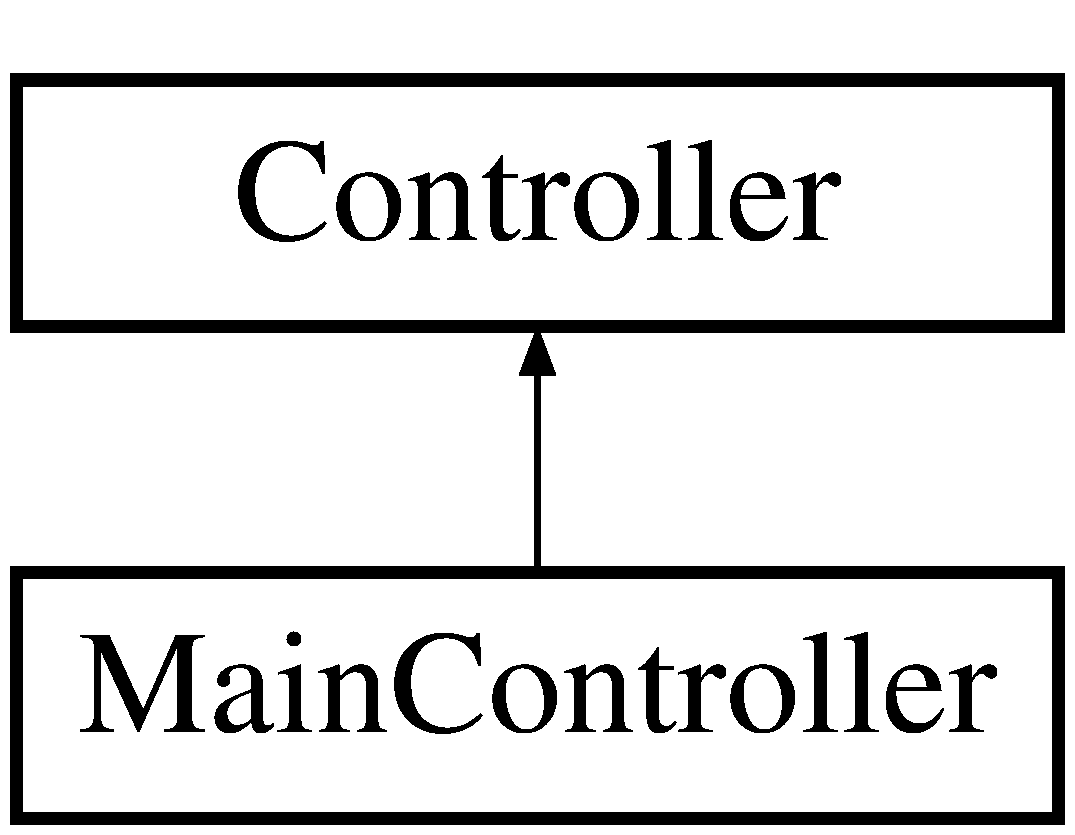
\includegraphics[height=2.000000cm]{class_main_controller}
\end{center}
\end{figure}
\subsection*{Открытые члены}
\begin{DoxyCompactItemize}
\item 
\mbox{\hyperlink{class_main_controller_acec97760f70f518bf7d237af380c7255}{Main\+Controller}} (std\+::shared\+\_\+ptr$<$ \mbox{\hyperlink{class_data_provider}{Data\+Provider}} $>$ data\+\_\+provider, std\+::shared\+\_\+ptr$<$ \mbox{\hyperlink{class_data_processing}{Data\+Processing}} $>$ data\+\_\+processing, std\+::shared\+\_\+ptr$<$ \mbox{\hyperlink{class_core}{Core}} $>$ core)
\begin{DoxyCompactList}\small\item\em Конструктор класса \end{DoxyCompactList}\item 
\mbox{\Hypertarget{class_main_controller_a5988de20a9d4f3d84cb7e3dabe2f6eec}\label{class_main_controller_a5988de20a9d4f3d84cb7e3dabe2f6eec}} 
void \mbox{\hyperlink{class_main_controller_a5988de20a9d4f3d84cb7e3dabe2f6eec}{run}} () const override
\begin{DoxyCompactList}\small\item\em Функция для запуска сценария программы \end{DoxyCompactList}\end{DoxyCompactItemize}


\subsection{Подробное описание}
Основной класс контроллер управляющий ходом программы 

См. определение в файле Controller.\+h строка 21



\subsection{Конструктор(ы)}
\mbox{\Hypertarget{class_main_controller_acec97760f70f518bf7d237af380c7255}\label{class_main_controller_acec97760f70f518bf7d237af380c7255}} 
\index{Main\+Controller@{Main\+Controller}!Main\+Controller@{Main\+Controller}}
\index{Main\+Controller@{Main\+Controller}!Main\+Controller@{Main\+Controller}}
\subsubsection{\texorpdfstring{Main\+Controller()}{MainController()}}
{\footnotesize\ttfamily Main\+Controller\+::\+Main\+Controller (\begin{DoxyParamCaption}\item[{std\+::shared\+\_\+ptr$<$ \mbox{\hyperlink{class_data_provider}{Data\+Provider}} $>$}]{data\+\_\+provider,  }\item[{std\+::shared\+\_\+ptr$<$ \mbox{\hyperlink{class_data_processing}{Data\+Processing}} $>$}]{data\+\_\+processing,  }\item[{std\+::shared\+\_\+ptr$<$ \mbox{\hyperlink{class_core}{Core}} $>$}]{core }\end{DoxyParamCaption})\hspace{0.3cm}{\ttfamily [inline]}}



Конструктор класса 


\begin{DoxyParams}{Аргументы}
{\em data\+\_\+provider} & Указатель на используемый провайдер \\
\hline
{\em data\+\_\+processing} & Указатель на используемый предобработчик данных \\
\hline
{\em core} & Указатель на используемое ядро \\
\hline
\end{DoxyParams}


См. определение в файле Controller.\+h строка 34



Объявления и описания членов класса находятся в файле\+:\begin{DoxyCompactItemize}
\item 
Controllers/Controller.\+h\end{DoxyCompactItemize}

\hypertarget{class_message}{}\section{Класс Message}
\label{class_message}\index{Message@{Message}}


{\ttfamily \#include $<$Message.\+h$>$}

\subsection*{Открытые члены}
\begin{DoxyCompactItemize}
\item 
\mbox{\Hypertarget{class_message_a4d3bec2b8b4a60d0a2505cab71ac43c6}\label{class_message_a4d3bec2b8b4a60d0a2505cab71ac43c6}} 
{\bfseries Message} (std\+::vector$<$ char $>$ lable, std\+::vector$<$ char $>$ message, float first\+\_\+class=0, float second\+\_\+class=0)
\item 
\mbox{\Hypertarget{class_message_a4a0a3ab72f842da9bba77242dcc233ba}\label{class_message_a4a0a3ab72f842da9bba77242dcc233ba}} 
std\+::vector$<$ char $>$ {\bfseries get\+\_\+lable} ()
\item 
\mbox{\Hypertarget{class_message_a19405ffc1c8399841f169751d3253ed7}\label{class_message_a19405ffc1c8399841f169751d3253ed7}} 
std\+::vector$<$ char $>$ {\bfseries get\+\_\+massage} ()
\item 
\mbox{\Hypertarget{class_message_a4785ba800ecde9660a97bd8f33293094}\label{class_message_a4785ba800ecde9660a97bd8f33293094}} 
void {\bfseries get\+\_\+massage} (std\+::vector$<$ char $>$ message)
\item 
\mbox{\Hypertarget{class_message_a255fb6f094bfaab61209d63408e5117e}\label{class_message_a255fb6f094bfaab61209d63408e5117e}} 
float {\bfseries get\+\_\+first\+\_\+class} ()
\item 
\mbox{\Hypertarget{class_message_adbdba18d32b805be4fe2d48475514edc}\label{class_message_adbdba18d32b805be4fe2d48475514edc}} 
void {\bfseries set\+\_\+first\+\_\+class} (float first\+\_\+class)
\item 
\mbox{\Hypertarget{class_message_a25bbcd4288aba998f403fb822fe05a98}\label{class_message_a25bbcd4288aba998f403fb822fe05a98}} 
float {\bfseries get\+\_\+second\+\_\+class} ()
\item 
\mbox{\Hypertarget{class_message_a63777d2455e6ab75eda2d802e0b365c9}\label{class_message_a63777d2455e6ab75eda2d802e0b365c9}} 
void {\bfseries get\+\_\+second\+\_\+class} (float second\+\_\+class)
\end{DoxyCompactItemize}


\subsection{Подробное описание}
Пример структуры данных. Лучше конечно использовать json. Либо сделать через интерфейсы эту структуру данных и тогда можно будет легко подключать различные структуры. 

См. определение в файле Message.\+h строка 11



Объявления и описания членов класса находятся в файле\+:\begin{DoxyCompactItemize}
\item 
Data\+Types/Message.\+h\end{DoxyCompactItemize}

%--- End generated contents ---

% Index
\backmatter
\newpage
\phantomsection
\clearemptydoublepage
\addcontentsline{toc}{chapter}{Алфавитный указатель}
\printindex

\end{document}
